\clearpage
\section{点光源下的金属高光}

把一块橙色面板放在三盏灯下，保持底色、相机和灯的位置不动。中图和右图都是金属，右图的表面更光滑。沿面板上半部寻找最亮的一点，粗糙表面把光反射到较宽的一片方向，光滑表面把它集中到较窄的一束。灯罩、金属把手和漆面会因此显出不同的质感。

\begin{center}
\begin{tabular}{@{}ccc@{}}
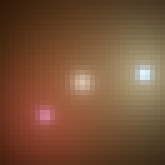
\includegraphics[width=.22\linewidth]{../../../output/profiling/point-materials/dielectric.png}&

\includegraphics[width=.22\linewidth]{../../../output/profiling/point-materials/rough-metal.png}&
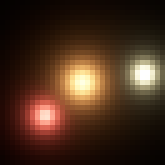
\includegraphics[width=.22\linewidth]{../../../output/profiling/point-materials/smooth-metal.png}\\
{\small 非金属，粗糙度 0.25}&{\small 金属，粗糙度 0.70}&{\small 金属，粗糙度 0.25}
\end{tabular}
\end{center}

这组三灯实测在 Vulkan 画出 $33\times33$ 个像素，三幅图使用相同曝光。正中像素的线性红通道依次为 1.170、0.346、16.105。最后一个数超过 1，着色器仍要保留它，显示时才压到屏幕能表现的亮度。若只拿底色乘光强，这三张图就无法区分。

设从面板指向灯、眼睛的单位向量分别为 $l,v$，表面法线为 $n$。能把这盏灯直接反进眼睛的小镜面朝向 $h=(l+v)/\lVert l+v\rVert$。GGX 用 $D$ 描述多少小镜面朝向 $h$，用 $G$ 描述其中有多少能同时看见灯和眼睛。粗糙度 $r$ 决定 $D$ 的宽度。代码取 $\alpha=\max(r^2,0.002)$，让最光滑的材质仍有一个有限宽度的高光；0.002 是项目的数值下限。$F$ 是光在这次反射中留下的比例，会随角度改变。光垂直照在普通非金属上时，glTF 取 $F_0=0.04$；金属则用自己的底色作 $F_0$。镜面反射函数为
\[
 f_s=\frac{D(h)\,G(l,v)\,F(v,h)}{4(n\cdot l)(n\cdot v)}.
\]
当前点落在灯的正面、且能看见灯时，把镜面与漫反射两项相加，再乘 $n\cdot l$ 和到达此点的灯光。点光源的强度随距离平方衰减，接近组件设定的半径时平滑降到零。分簇绘制先剔除照不到这里的灯，对留下的灯仍查相同的阴影、使用同一反射公式。

glTF 粗糙度贴图的绿色通道保存粗糙度，蓝色保存金属度。比如绿色的字节值为 64，粗糙度因子为 0.8，着色时取 $0.8\times64/255=0.201$。这两个通道都直接除以 255，底色贴图才需要从 sRGB 解码。DDGI 只传播漫反射，用 $(1-m)c$ 表示金属度 $m$、底色 $c$ 的漫反射率。在两面墙的测试里，经过两墙到达相机的红光为 0.277；将反光墙或接收墙分别换成纯金属，这项都降为零。

{\small\href{https://registry.khronos.org/glTF/specs/2.0/glTF-2.0.html\#appendix-b-brdf-implementation}{glTF 2.0 附录 B}\quad
\href{https://pbr-book.org/4ed/Reflection_Models/Roughness_Using_Microfacet_Theory}{PBRT 第四版 §9.6}\quad
\href{run:../../Redflag/src/Redflag/Renderer/GI/Shaders/PointLighting.glsl}{点光源着色源码}\quad
\href{run:../profiling/point-materials/README.md}{原图、实测与操作方法}}
